
\chapter{Two simple examples}
We give two detailed examples that will exemplify the mechanics of the GUI. For clarity we will use colour boxes that will exemplify the window that we refer to. So green boxes refer to the processed window, yellow ones to the input window and gray ones to the feedback window.

\subsection{Propositional Calculus}

We will prove that if $P$ and $Q$ are propositions then $$P\lor Q \Rightarrow Q\lor P$$

the way to enter this is:

\inp{Lemma commor(P Q :Prop): P \texttt{\char`\\}/ Q -> Q \texttt{\char`\\}/ P .}
 
 Note that  the feedback from Coq says 
\coq{
P,  Q : Prop \\
}{
P  \lor  Q  \rightarrow  Q \lor  P 
}
This means that the hypotheses are that $P$ and $Q$ are propositions and the conclusion is $ P \lor Q \rightarrow Q \lor P$. To prove an implication  statement we assume the left hand and try to prove the right hand. Here is how you do it in Spatchcoq. There are two different ways to do this in spatchCoq:

Type ``Assume'' and press ESC to get a list of tactic choices:

\begin{figure}[h!]

\includegraphics[scale=0.5]{Installation/Escape.png}


\label{tactics}
\end{figure}

choose the tactic

\noindent
\inp{Assume VAR then prove VAR.}

Press \VAR to select the first VAR.

write $( P \lor Q )$ to replace the first VAR. Repeat \VAR and and replace the second VAR by $(Q \lor P)$.



The text in the yellow window should now be 

\noindent
\inp{Assume $( P \lor Q )$ then prove $( Q \lor P )$.}

Click run.


The other variant is to click on the orange goal in the feedback column to get a number of  to get a list of possible choices:
\begin{figure}[h!]
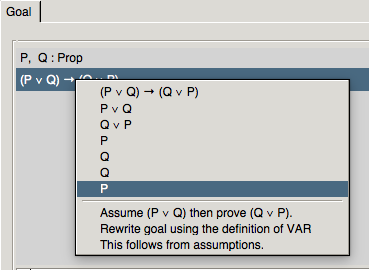
\includegraphics[scale=0.5]{Installation/clickgoal.png}
\label{tactics}
\end{figure}
Note that the choices bellow the horizontal line are tactics while those on the top are pieces of the goal. You can use a combination of the two methods of course. As before choose 
\inp{Assume $( P \lor Q )$ then prove $( Q \lor P )$.} and click run.


The response from Coq is

\coq{
 P \ Q: \mbox{Prop}\\
\mbox{Hyp}: P \lor Q
}{Q\lor P
}

This reflects the fact that we have a new hypothesis tabled Hyp  and a new conclusion.

Of course since we have a hypothesis with a disjunction we will use an argument by cases. To do so, type ``cases'' and press ESC. Choose the following:
\inp{Consider cases based on disjunction in hypothesis VAR.}

Press \VAR and replace VAR by Hyp. Click run.

Similarly click on the hypothesis Hyp on the right hand side to get:

\begin{figure}[h!]
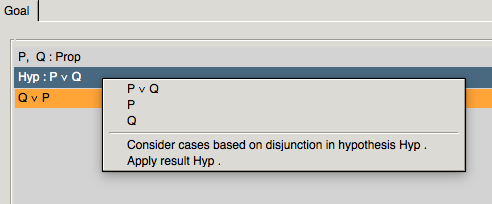
\includegraphics[scale=0.5]{Installation/clickgoal1.png}
\label{tactics}
\end{figure}
 choose 
\inp{Consider cases based on disjunction in hypothesis Hyp .}

and click Run.

Notice that there are now two goals:
\coq{
 P \ Q: \mbox{Prop}\\
\mbox{Hyp0}: P\\
===========\\
}{
Q\lor P
}

and 

\coq{
P \ Q: \mbox{Prop}\\
\mbox{Hyp1}:  Q\\
===========
}{
Q\lor P
}

corresponding to the two cases to consider. In first goal we will prove the right hand side of the disjunction in the conclusion. To do so, type ``right'' and press ESC. You get to pick

\inp{
Prove right hand side.}

and after clicking run you will get the following feedback (note that the second goal stays unchanged)

\coq{
P \ Q: \mbox{Prop}\\
\mbox{Hyp0}: P\\
===========
}{
 P
}

Finally you can finish this goal by using the hypothesis Hyp0. To do this you use
\inp{This follows from assumptions.}

Note that you have now finished this goal. Repeat the argument for the second goal by using:

\inp{Prove left hand side.}
\inp{This follows from assumptions.}

to get \coq{ }{\text{no goals}}

Now type
\inp{Qed.}
to save the theorem. It now appears among the proved theorems:

and you can see its proof tree by clicking on draw tree:


\begin{figure}[h!]
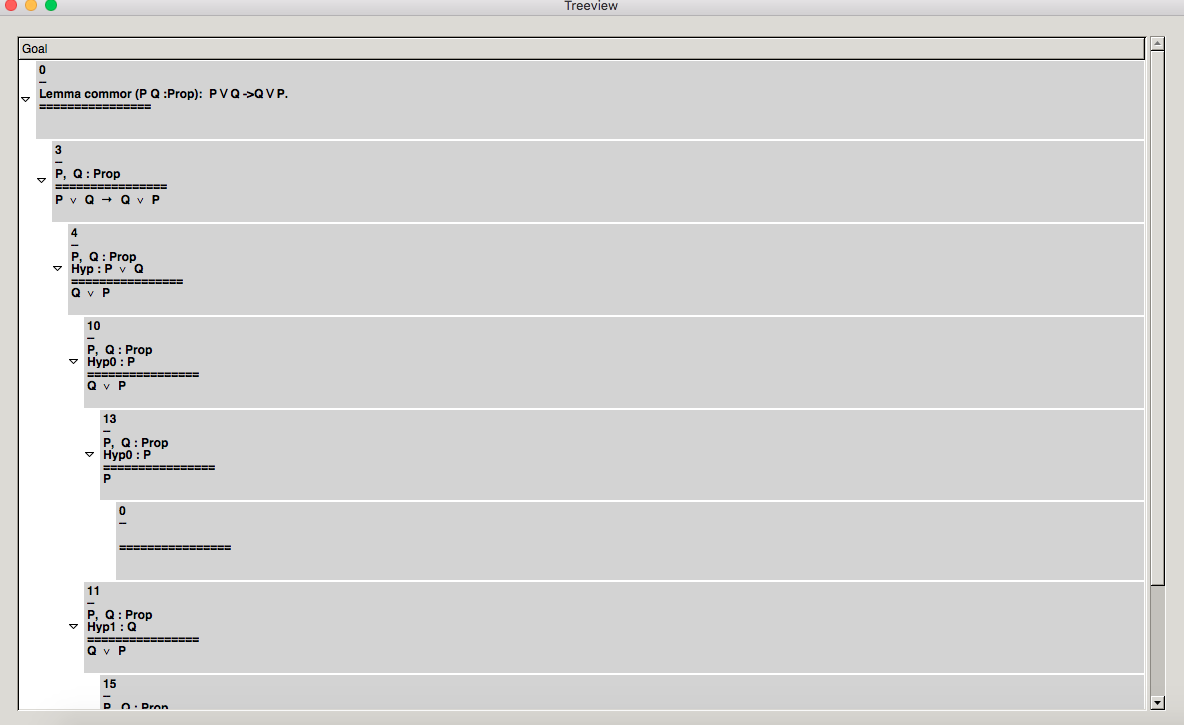
\includegraphics[scale=0.3]{Installation/treecommor.png}
\caption{the tree window}\label{treesearch}
\end{figure}

\subsection{An elementary number theory example}
We shall prove the transitivity of divisibility. That is we will prove that
$$\forall a,b, c \in \mathbb{N},  a |b \land b | c \Rightarrow a | c.$$

In the process we will introduce definitions and notations.

To start we note that we will be talking about objects of type \texttt{nat}. We weill introduce the following definition

\inp{Definition divides a b := exists x:nat, b = a*x.}

We hope that the format is quite clear, it resembles the one we used before but uses a few new notions, the operator \texttt{:=}
 which the defines the function \texttt{divides} and the quantifier \texttt{exists}. Note that we have not explicitly stated that a and b should be natural numbers, Coq will deduce that from the context. We could have been very precise as follows:
 \inp{ Definition divides (a b:nat) := exists x:nat, b = a*x.}

Note that the definition will not get any feedback from Coq. If we want to check that we have correctly defined our notion we can use
\inp{Check divides.}

to get

\mess{Query commands should not be inserted in
scripts\\

divides\\
     \texttt{: nat -> nat -> Prop}}
     
or
\inp{Print divides.}
to get a more detailed 
\mess{
Query commands should not be inserted in
scripts \\

divides = $\lambda a b : nat, \exists x : nat, b = a * x$\\
    \texttt{ : nat -> nat -> Prop}
\\
Argument scopes are [nat\_scope nat\_scope]
}
We will nod describe all this output here but we note the change from \texttt{exists} to $\exists$ and the occurrence of $\lambda$, a notation for functions.


Next we define a notation for divides

\inp{Notation " a | b " := (divides a b) (at level 10).}

Again no feedback from Coq. The definition should be self-evident except for the ``(at level 10)'' part. We will discuss this elsewhere.

We are now ready to state out theorem

We can state the theorem as (see the corresponding feedback)

\inp{Theorem refldiv (a b c:nat): \\ (a | b) $\land$ (b | c) -> (a |c).}

\coq{a,  b,  c : nat }{a  |  b  \land  b  |  c \rightarrow  a  |  c }

but we prefer the version

\inp{Theorem refldiv: forall a b c, (a | b) $\land$ (b | c) -> (a |c).
}
because it is  almost identical to the above mathematical statement and it will allow us to show some more tactics. The corresponding feedback is
\coq{ }{
\forall  a \  b\   c : nat,  a  |  b \  \land \ b  |  c\  \rightarrow\ a  |  c }

Note that Coq has correctly deduced that $a, b, c$ are natural numbers and replaced the quantifier \texttt{forall} with $\forall$. Note also that in this form there are no hypotheses.

We fill fix the three variables with the tactics:
\inp{Fix an arbitrary element a.\\
Fix an arbitrary element b.\\
Fix an arbitrary element c.}

to get 
\coq{a,  b,  c : nat \\
}{
a  |  b  \land  b  |  c \rightarrow  a  |  c }

As before, in order to prove an implication $A\rightarrow B$ we use the tactic

\inp{Assume A then prove B.}

More precisely, in this case we have
\inp{Assume (a | b $\land$ b | c ) then prove (a | c).}
to get

\coq {a,  b,  c : nat \\
Hyp : a  |  b  \land  b  |  c \\
}{
a  |  c }


Note that hypothesis Hyp is of type $A \land B$. We will split this in two hypotheses with:
\inp{Eliminate the conjuction in hypothesis Hyp.}
to get

\coq {a,  b,  c : nat \\
Hyp0 : a  |  b\\
Hyp1 :  b  |  c \\
}{
a  |  c }

We seem to have used all the tricks up our selves and so it is time to ``unfold'' the definitions:
\inp{Rewrite hypothesis Hyp0 using the definition of divides.}
\coq{a,  b,  c : nat \\
Hyp0 : \exists  x  :  nat,  b  =  a  *  x \\
Hyp1 :  b  |  c \\
}{
a  |  c }

then 
\inp{Rewrite hypothesis Hyp1 using the definition of divides.}
\coq{a,  b,  c : nat \\
Hyp0 : \exists  x  :  nat,  b  =  a  *  x \\
Hyp1 : \exists  x  :  nat,  c  =  b  *  x \\
}{
a  |  c }
and 

\inp{Rewrite goal using the definition of divides.}
\coq{a,  b,  c : nat \\
Hyp0 : \exists  x  :  nat,  b  =  a  *  x \\
Hyp1 : \exists  x  :  nat,  c  =  b  *  x \\
}{
\exists x : nat,  c  =  a  *  x  }


We now pick x as in the hypothesis Hyp1, that is:
\inp{Fix x the existentially quantified variable in Hyp1.}
to get 
\coq{a,  b,  c : nat \\
Hyp0 : \exists  x  :  nat,  b  =  a  *  x \\
x : nat \\
Hyp1 :   c  =  b  *  x \\
}{
\exists x0 : nat,  c  =  a  *  x0  }

Note the variable name was changed in the goal but not in Hyp0.

We now use the newly formed Hyp1 as follows:

\inp{Rewrite the goal using Hyp1.}

to get
\coq{a,  b,  c : nat \\
Hyp0 : \exists  x  :  nat,  b  =  a  *  x \\
x : nat \\
Hyp1 :   c  =  b  *  x \\
}{
\exists x0 : nat,  b  *  x  =  a  *  x0  }

Similarly we pick y as in Hyp0 and replace it in the goal

\inp{
Fix y the existentially quantified variable in Hyp0.\\
Rewrite the goal using Hyp0.
}

to get

\coq{a,  b,  c y : nat \\
Hyp0 :   b  =  a  *  y \\
x : nat \\
Hyp1 :   c  =  b  *  x \\
}{
\exists x0 : nat,  a  *  y  *  x  =  a  *  x0  }


It is now easy to guess that $x0 = y*x$ so we write

\inp{Prove the existential claim is true for (y*x).}

to obtain

\coq{a,  b,  c y : nat \\
Hyp0 :   b  =  a  *  y \\
x : nat \\
Hyp1 :   c  =  b  *  x \\
}{
 a  *  y  *  x  =  a  *  (y*x)  }

which can be proved by

\inp{True by arithmetic properties.}


the total proof is
\inp{
Definition divides (a b:nat) := exists x:nat, b = a*x. \\
Notation " a | b " := (divides a b) (at level 10).\\
Theorem refldiv:forall a b c, (a | b) $\land$ (b | c) -> (a |c).\\
Fix an arbitrary element a.\\
Fix an arbitrary element b.\\
Fix an arbitrary element c.
Assume (a | b $\land$ b | c ) then prove (a | c).\\
Eliminate the conjuction in hypothesis Hyp.\\
Rewrite hypothesis Hyp0 using the definition of divides.\\
Rewrite hypothesis Hyp1 using the definition of divides.\\
Rewrite goal using the definition of divides.\\
Fix x the existentially quantified variable in Hyp1.\\
Rewrite the goal using Hyp1.\\
Fix y the existentially quantified variable in Hyp0.\\
Rewrite the goal using Hyp0.\\
Prove the existential claim is true for (y*x).\\
True by arithmetic properties.
}

Note that one could use a slightly shorter version of this theorem:


\inp{Theorem refldiv (a b c:nat): (a | b) $\land$ (b | c) -> (a |c).\\
Rewrite goal using the definition of divides.\\
Assume $((\exists  x : nat,  b  =  a  *  x)  \land  (\exists  x  :  nat,  c  =  b  *  x)  )$ then prove $( \exists  x  :  nat,  c  =  a  *  x)$.\\
Eliminate the conjuction in hypothesis Hyp.\\
Fix x the existentially quantified variable in Hyp1.\\
Rewrite the goal using Hyp1.\\
Fix y the existentially quantified variable in Hyp0.\\
Rewrite the goal using Hyp0.\\
Prove the existential claim is true for (y*x).\\
True by arithmetic properties.}



Note also that if you save the latex form of the proof you will obtain the following:
\begin{tcolorbox}[colback=gray!10!white,colframe=white,breakable]
\begin{Definition}[divides] 
$divides\,(a\,b:nat)\,:=\,∃\,x:nat,\,b\,=\,a*x.
$
 \end{Definition}
\begin{Theorem}[refldiv] 
$\forall \,a\,b\,c,\,(a\,|\,b)\,\land (b\,|\,c)\,\Rightarrow \,(a\,|c).$
 \end{Theorem}
 Proof: In order to show $$\forall a b c : nat, a | b \land b | c \Rightarrow a | c $$ we pick an arbitrary $$a$$ and show $$\forall b c : nat, a | b \land b | c \Rightarrow a | c .$$
 In order to show $$\forall b c : nat, a | b \land b | c \Rightarrow a | c $$ we pick an arbitrary $$b$$ and show $$\forall c : nat, a | b \land b | c \Rightarrow a | c .$$
 In order to show $$\forall c : nat, a | b \land b | c \Rightarrow a | c $$ we pick an arbitrary $$c$$ and show $$a | b \land b | c \Rightarrow a | c .$$

 

 We will assume $$Hyp : a | b \land b | c $$ and show $$a | c .$$

 Since we know $$Hyp : a | b \land b | c $$ we also know $$Hyp0 : a | b 
Hyp1 : b | c .$$

 We use the definition of $$divides$$ in $$Hyp0$$ to obtain $$Hyp0 : \exists x : nat, b = a * x $$ 

 We use the definition of $$divides$$ in $$Hyp1$$ to obtain $$Hyp1 : \exists x : nat, c = b * x $$ 

 Rewriting the definition of $$divides$$ in our conclusion $$a | c $$, we now need to show $$\exists x : nat, c = a * x .$$

 We choose a variable $$x$$ in $$Hyp1$$ to obtain $$x : nat 
Hyp1 : c = b * x .$$

 We rewrite the goal using $$Hyp1$$ to obtain $$\exists x0 : nat, b * x = a * x0 .$$

 We choose a variable $$y$$ in $$Hyp0$$ to obtain $$a, b, c, y : nat 
Hyp0 : b = a * y .$$

 We rewrite the goal using $$Hyp0$$ to obtain $$\exists x0 : nat, a * y * x = a * x0 .$$

 We shall prove $$\exists x0 : nat, a * y * x = a * x0 $$ by showing $$a * y * x = a * (y * x) .$$

 This follows immediately from arithmetic.

 This is done Now $$a * y * x = a * (y * x) $$ means that $$\exists x0 : nat, a * y * x = a * x0 .$$ We have now proved $$\exists x0 : nat, a * y * x = a * x0 $$ and so $$\exists x0 : nat, b * x = a * x0 $$ follows. and so we have proved $$\exists x0 : nat, b * x = a * x0 .$$ We have now proved $$\exists x0 : nat, b * x = a * x0 $$ and so $$\exists x0 : nat, c = a * x0 $$ follows. and so we have proved $$\exists x : nat, c = a * x .$$ Therefore we have showed $$\exists x : nat, c = a * x $$ and so $$a | c .$$ therefore we have $$a | c .$$ therefore we have $$a | c .$$ We are now done with $$a | c .$$ We have now showed that if $$Hyp : a | b \land b | c $$ then $$a | c $$ a proof of $$a | b \land b | c \Rightarrow a | c .$$ Since $$c$$ was arbitrary this shows $$\forall c : nat, a | b \land b | c \Rightarrow a | c .$$ Since $$b$$ was arbitrary this shows $$\forall b c : nat, a | b \land b | c \Rightarrow a | c .$$ Since $$a$$ was arbitrary this shows $$\forall a b c : nat, a | b \land b | c \Rightarrow a | c .$$
 

\end{tcolorbox}
